% Copyright 2021 Edoardo Riggio

% Licensed under the Apache License, Version 2.0 (the "License");
% you may not use this file except in compliance with the License.
% You may obtain a copy of the License at

% 	http://www.apache.org/licenses/LICENSE-2.0

% Unless required by applicable law or agreed to in writing, software
% distributed under the License is distributed on an "AS IS" BASIS,
% WITHOUT WARRANTIES OR CONDITIONS OF ANY KIND, either express or implied.
% See the License for the specific language governing permissions and
% limitations under the License.

\documentclass{article}

\usepackage{hyperref, amsmath, graphicx, amssymb, csquotes}
\usepackage{fancyvrb,newverbs,xcolor}

\graphicspath{ {./assets/} }

\definecolor{cverbbg}{gray}{0.93}

\newenvironment{cverbatim}
 {\SaveVerbatim{cverb}}
 {\endSaveVerbatim
  \flushleft\fboxrule=0pt\fboxsep=.5em
  \colorbox{cverbbg}{\BUseVerbatim{cverb}}%
  \endflushleft
}

\newenvironment{lcverbatim}
 {\SaveVerbatim{cverb}}
 {\endSaveVerbatim
  \flushleft\fboxrule=0pt\fboxsep=.5em
  \colorbox{cverbbg}{%
    \makebox[\dimexpr\linewidth-2\fboxsep][l]{\BUseVerbatim{cverb}}%
  }
  \endflushleft
}

\newcommand{\ctexttt}[1]{\colorbox{cverbbg}{\texttt{#1}}}
\newverbcommand{\cverb}
  {\setbox\verbbox\hbox\bgroup}
  {\egroup\colorbox{cverbbg}{\box\verbbox}}

\begin{document}
\begin{titlepage}
    \begin{center}
        \vspace*{1cm}
        
        \Huge
        \textbf{Artificial Intelligence Cheatsheet}
        
        \vspace{0.5cm}
        \LARGE
        
        \vspace{.5cm}
        
        Edoardo Riggio
   		  \vspace{1.5cm}
       
        \vfill
        
        \today
        
        \vspace{.8cm}
          \Large
          Artificial Intelligence - SA. 2021 \\
        Computer Science\\
        Universit\`{a} della Svizzera Italiana, Lugano\\
        
    \end{center}
\end{titlepage}

\tableofcontents

\newpage

\section{Blind Search Algorithms}
A \textbf{search algorithm} takes as input a problem space and a starting state, and tries to compute a path in the best possible way. \\ \\
The strategy is to search which node to expand among the yet undiscovered nodes. In order to expand a node, we need to consider all of the nodes that are reachable in one step from the selected node.

\subsection{Definitions}
\subsubsection{Search Tree}
A search tree is a tree composed of nodes. Each node in the tree represents a step in the search algorithm. A node is composed of:

\begin{itemize}
	\item State
	\item Node who generated it
	\item Action used to generate it
	\item Depth of the tree
	\item Cost of the path from the root
\end{itemize}

\subsubsection{Travelling Salesman Problem}
The goal of this problem is to visit all the cities of a graph such that the travelling cost is minimum. The travelling cost is measured by summing up all of the travelling costs from the starting city to the destination city.

\subsubsection{Evaluation of Search Strategies}
There are four common criteria for evaluating search strategies:

\begin{itemize}
	\item \textbf{Completeness}
	\vspace{.2cm} \\
	Does the algorithm always find a solution if one exists?
	
	\item \textbf{Optimality}
	\vspace{.2cm} \\
	Does the algorithm guarantee the least-cost solution?
	
	\item \textbf{Time Complexity}
	\vspace{.2cm} \\
	How much time does it take for an algorithm to run?
	
	\item \textbf{Space Complexity}
	\vspace{.2cm} \\
	How much memory does the algorithm require?
\end{itemize}

\subsection{Breath-First Search}
In this algorithm, the shallowest unexpanded node is expanded. In order to do so, this algorithm requires a FIFO queue. This type of queue is able to keep track of which node to expand next. \\

\begin{center}
	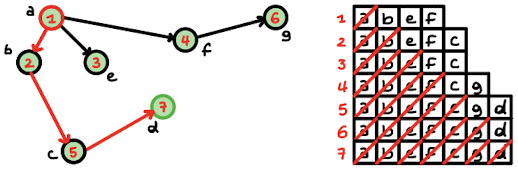
\includegraphics[width=9cm]{bfs.png}
\end{center}
\vspace{.3cm}
This algorithm is \textbf{complete}. It is also \textbf{optimal} in the case that all of the steps have the same cost. Furthermore, the \textbf{space and time complexities} of this algorithm are both $O(b^d)$. Where $b$ is the branching factor, and $d$ is the solution depth.

\subsection{Uniform-Cost Search}
In this algorithm, a cost is assigned to each edge of the graph. Here a node is expanded if $g(n)$ -- i.e. the distance from the root to the node -- is minimal. \\

\begin{center}
	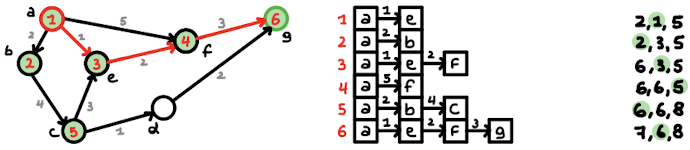
\includegraphics[width=12cm]{ucs.png}
\end{center}
\vspace{.3cm}
In the above image, on the far right we have the values of $g(n)$ at each step, while in the middle, we have the path chosen at each step. \\ \\
This algorithm is \textbf{complete}. It is also \textbf{optimal} in the case that all costs are non-negative. Furthermore, the \textbf{space and time complexities} are both $O(b^d)$, where $b$ is the branching factor, and $d$ is the solution depth.

\subsection{Depth-First Search}
This algorithm expands the deepest unexpanded node. In order to do so, it uses a LIFO queue. \\

\begin{center}
	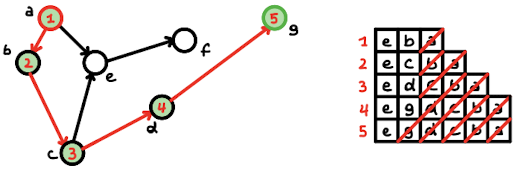
\includegraphics[width=9cm]{dfs.png}
\end{center}
\vspace{.3cm}
This algorithm is \textbf{not complete} in the case of an infinite state space -- since it has no depth limitation. It is also \textbf{not optimal}. Furthermore, the \textbf{time complexity} of the algorithm is $O(b^m)$, while the \textbf{space complexity} is $O(b \cdot m)$. Where $b$ is the branching factor and $m$ is the maximum depth of the search tree.

\subsection{Depth-Limited Search}
In this case we have an algorithm which is identical to the DFS search. The only difference between the two is that depth-limited search is -- as the name suggests -- limited. This means that it will stop when it reaches a certain depth in the solution tree. \\ \\
This algorithm is \textbf{complete} in the case where we know a bound to the solution depth. It is \textbf{not optimal}. Furthermore, the \textbf{time complexity} is $O(b^d)$, and the \textbf{space complexity} is $O(b \cdot d)$. Where $b$ is the branching factor and $d$ is the maximum depth.

\subsection{Iterative Deepening Search}
This is a depth-limited search algorithm, where at each step, a counter representing the tree's depth is incremented. DFS is performed at every repetition of the algorithm -- when the algorithm goes back to the starting node, and it stops at the depth indicated by the counter. \\ \\
This algorithm is \textbf{complete}. It is also \textbf{optimal} in the case that there are non-negative costs. Furthermore, the \textbf{time complexity} is $O(b^d)$, and the \textbf{space complexity} is $O(b \cdot d)$. Where $b$ is the branching factor and $d$ is the depth at which the goal is found.

\subsection{Bi-Directional Search}
This algorithm considers two queues, one only containing the root, and one only containing the goal. The nodes of each queue are expanded until both queues contain a common node. \\ \\
This algorithm is both \textbf{complete} and \textbf{optimal}. Furthermore, the \textbf{time and space complexities} are $O(b ^{\frac{d}{2}})$, where $b$ is the branching factor, and $d$ is the depth at which the goal is located.

\section{Heuristic Search Algorithms}
\textbf{Heuristic knowledge} helps to execute good choices. It does not avoid search, but it reduces it. It is used when a problem has exponential complexity -- i.e. is NP-complete. \\ \\
This knowledge is given by a state evaluation function, called the \textbf{heuristic evaluation}.

\subsection{Definitions}
\subsubsection{Admissible Heuristic}
A heuristic is said to be admissible if it never overestimates the cost of reaching the goal -- i.e. the cost estimated to reach the goal is not higher than the lowest possible cost from the current node.

\[ \forall n~|~h(n) \leq h^*(n) \] \\
Where $n$ is a node, $h$ is a heuristic, $h(n)$ is the cost from node $n$ to the goal -- defined by $h$, and $h^*(n)$ is the optimal cost from $n$ to the goal.

\subsubsection{Monotonic Heuristic}
A heuristic is said to be monotone if, for each node $n$ and its successor $n'$, the estimated cost of reaching the goal from $n$ is no longer greater than the step cost of getting to $n'$ plus the estimated cost of reaching the goal from $n'$.

\[ f(n) \leq f(n') \] \\
Where $f(n)$ is the cost from the root to node $n$ plus the cost estimation from node $n$ to the goal. Same thing goes for $f(n')$. A monotonic heuristic is always admissible. Not all admissible heuristics are monotonic. In addition, all monotonic heuristics guarantee local optimality.

\subsection{Best First Search}
Each node of the graph is evaluated by estimating its distance to the goal. The node which has the shortest distance to the goal is selected to be expanded.\\

\begin{center}
	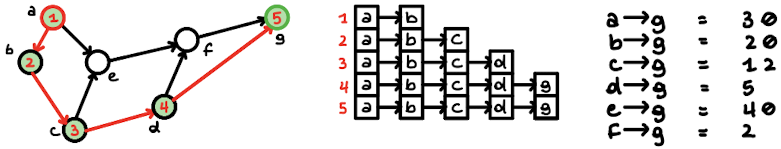
\includegraphics[width=12cm]{befs.png}
\end{center}
\vspace{.3cm}
Where on the far right we have all the values given by the heuristic function $h$. \\ \\
This algorithm is \textbf{not complete} and \textbf{not optimal}. Furthermore, the \textbf{time complexity} and \textbf{space complexity} are both $O(b^m)$. Where $b$ is the branching factor and $m$ is the depth of the search tree.

\subsection{A*}
The evaluation function for this algorithm is:

\[ f^*(n) = g^*(n) + h^*(n) \] \\
Where $f^*(n)$ is the estimated cost of the path from the root to the goal, $g^*(n)$ is the cost of the path from the root to node $n$, and $h^*(n)$ is the estimated cost of the path from node $n$ to the goal -- given by the heuristic $h$.\\

\begin{center}
	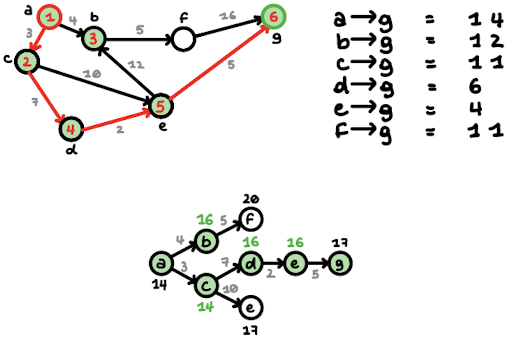
\includegraphics[width=9cm]{a*.png}
\end{center}
\vspace{.3cm}
This algorithm is \textbf{complete} -- unless there are infinitely many nodes with $f \leq f(G)$, where $G$ is the goal. It is also \textbf{optimal}. Furthermore, the \textbf{time complexity} and \textbf{space complexity} are both $O(b^m)$. Where $b$ is the branching factor and $m$ is the depth of the search tree.

\subsubsection{Optimality of A*}
Given that: \blockquote{If $A^*$ selects a path $p$, then $p$ is the shortest path -- i.e. least-cost path -- in order to reach the goal}, the optimality of $A^*$ can be demonstrated in the following way:

\begin{enumerate}
	\item Assume -- for contradiction -- that some other path $p'$ is actually the shortest path to a goal
	\item Consider that, before $p$ is chosen from the fringe, some part of path $p'$ will also be on the fringe. This partial path will be called $p''$
	\item Because $p$ was expanded before $p''$ was, then we will have:
	\[ f(p) \leq f(p'') \]
	\item Because $p$ is a goal, this means that $h(p) = 0$. Thus:
	\[ g(p) \leq g(p'') + h(p'') \]
	\item Because $h$ is admissible, this means that the following is true for any path $p'$ to a goal that extends $p''$:
	\[ g(p'') + h(p'') \leq g(p') \]
	\item We will thus obtain the following for any other path $p'$ to a goal:
	\[ g(p) \leq g(p') \]
	Which contradicts the assumption of $p'$ being the shortest path
\end{enumerate}

\subsection{IDA*}
This algorithm combines $A^*$ with iterative deepening. At each iteration of the algorithm, we perform DFS, pruning the branches in which its total estimated cost

\[ f(n) = g(n) + h(n) \] \\
Exceeds a given threshold. The value of this threshold starts as the value of $f$ of the initial node, and increases for each iteration of the algorithm. The next value of the threshold is computed as the minimum value of $f$ of all values that exceeded the current threshold. \\ \\
As for $A^*$, this algorithm is also both \textbf{complete} and \textbf{optimal}. Furthermore, the \textbf{time complexity} is $O(b^m)$, while the \textbf{space complexity} is $O(b \cdot d)$.

\section{Constructive Greedy Search Algorithms}
A constructive greedy algorithm is based on the following steps:

\begin{enumerate}
	\item Start from a random node
	\item Expand the node in order to generate all possible next nodes
	\item Choose the next best node based on a local strategy
	\item Current solution is extended with the one found at point 3
	\item Repeat steps 2 through 4, until a feasible solution is computed
\end{enumerate}
These algorithms start from a feasible solution in a subset of the search space, and iteratively add elements to the partial solution -- according to some strategy -- until no node is left.

\subsection{Nearest Neighbour}
This is one of the most common algorithms used to solve TSP problems. The algorithm is the following:

\begin{enumerate}
	\item Consider a starting tour made up of a random node
	\item Add the city which is the closest to the previous city to the tour. The next city must not have been visited yet
	\item Repeat step 2 until no node is available
\end{enumerate}
The following is a graphical representation of the algorithm.\\

\begin{center}
	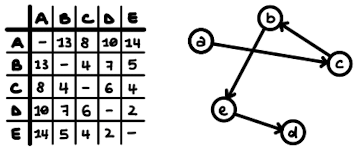
\includegraphics[width=6cm]{nn.png}
\end{center}
\vspace{.3cm}
Where on the right we have the connectivity matrix of the graph. Each non-zero element in the matrix represents the distance between two nodes $n_i$ and $n_j$. \\ \\
The \textbf{time complexity} of this algorithm is $O(n^2)$.

\subsection{Multi-Fragment}
This algorithm builds a tour as follows:

\begin{enumerate}
	\item Sort the edge costs in ascending order
	\item Select the first edge. This will be the first edge of the new tour
	\item Add new edge in incremental order only if it does not create a three-degree city -- i.e. does not create a cycle
	\item Repeat step 3 until no edge is available
\end{enumerate}
The \textbf{time complexity} of this algorithm is $O(n^2 \cdot \log n)$.

\subsection{Nearest Insertion}
This algorithm does the following:

\begin{enumerate}
	\item Build an initial tour formed by the nearest cities
	\item Choose a node that is not in the computed tour, such that the Euclidean distance between it and two other nodes in the tour is minimum
	\item Insert the new node between the two nodes of the tour
	\item Repeat steps 2 and 3 until there are no nodes left
\end{enumerate}
The \textbf{time complexity} of this algorithm is $O(n^2)$.

\subsection{Farthest Insertion}
This algorithm does the following:

\begin{enumerate}
	\item Build an initial tour formed by the farthest cities
	\item Choose a node that is not in the computed tour, such that the Euclidean distance between it and two other nodes in the tour is maximum
	\item Insert the new node between the two nodes of the tour
	\item Repeat steps 2 and 3 until there are no nodes left
\end{enumerate}
The \textbf{time complexity} of this algorithm is $O(n^2)$.

\end{document}






























 
